\documentclass[tombow,dvipdfmx]{corona-a5-1.1}
% dvipdfmxを追加(川口)

% Springer document settings
\usepackage[bottom]{footmisc}% places footnotes at page bottom

\usepackage{newtxtext}       % 
\usepackage[varvw]{newtxmath}       % selects Times Roman as basic font
%%%%%%%%%%%%%%%%%%%%%%%%%%%%%%%

% \usepackage{amssymb}
\usepackage{ntheorem}
\usepackage{amsmath}
\usepackage{enumitem}


\usepackage{graphicx}
\usepackage{color}
\usepackage{cite}
\usepackage{makeidx}


\usepackage{ascmac}
\usepackage{eclbkbox}
\usepackage{dsfont}

\usepackage{longtable}

\usepackage{url}

\usepackage{hyperref}

\usepackage{multicol}

%% --川口追加--
\makeatletter
\let\MYcaption\@makecaption
\makeatother
\usepackage{subcaption}
\captionsetup{compatibility=false}      % 必要に応じて

\makeatletter
\let\@makecaption\MYcaption
\makeatother
% ----

%%
\theoremstyle{plain}
\theoremheaderfont{\bfseries}
\theorembodyfont{\rmfamily}
\theoremseparator{\hspace{1ex}}
\theoremindent0cm
\theoremnumbering{arabic}
\theoremprework{\vspace{1ex}\begin{shadebox}\vspace{1ex}}
\theorempostwork{\vspace{-1ex}\end{shadebox}\vspace{1ex}}

%%
\theoremclass{theorem}

%%
\theoremclass{theorem}

%%
\theoremclass{theorem}


%%
\theoremstyle{break}
\theoremheaderfont{\bfseries}
\theorembodyfont{\rmfamily}
\theoremseparator{}
\theoremindent0cm
\theoremnumbering{arabic}
\theoremprework{\vspace{1.5ex}\begin{breakbox}\vspace{-0.5ex}}
\theorempostwork{\vspace{-0.5ex}\end{breakbox}\vspace{1.5ex}}

%%
\theoremstyle{nonumberplain}
\theoremseparator{\hspace{1ex}}

%%
\newtheorem{assumption}{Assumption}[section]

%%
\renewcommand{\theproblem}{}

\renewcommand{\theremark}{}


\newcommand{\red}[1]{{\color{red}#1}}
\newcommand{\blue}[1]{{\color{blue}#1}}
\newcommand{\green}[1]{{\color{green}#1}}

\DeclareMathOperator*{\argmax}{arg\,max}

\newcommand{\bm}[1]{\boldsymbol{#1}}
\newcommand{\sfT}{\mathsf{T}}

\newcommand{\advanced}{$^{\ddag}$}

\DeclareMathOperator{\sfsin}{\mathsf{sin}}
\DeclareMathOperator{\sfcos}{\mathsf{cos}}
\DeclareMathOperator{\sftan}{\mathsf{tan}}
\DeclareMathOperator{\sfarctan}{\mathsf{arctan}}

\DeclareMathOperator{\sfdiag}{\mathsf{diag}}
\DeclareMathOperator{\sfcol}{\mathsf{col}}
\DeclareMathOperator{\sfdet}{\mathsf{det}}
\DeclareMathOperator{\sfadj}{\mathsf{adj}}
\DeclareMathOperator{\sftrace}{\mathsf{trace}}

\DeclareMathOperator{\real}{\mathsf{Re}}

\DeclareMathOperator{\sfker}{\mathsf{ker}}
\DeclareMathOperator{\sfim}{\mathsf{im}}

\DeclareMathOperator{\sfdim}{\mathsf{dim}}
\DeclareMathOperator{\sfspan}{\mathsf{span}}

\DeclareMathOperator{\sfint}{\mathsf{int}}

\DeclareMathOperator*{\sfmin}{\mathsf{min}}
\DeclareMathOperator*{\sfmax}{\mathsf{max}}
\DeclareMathOperator*{\sfsup}{\mathsf{sup}}

\DeclareMathOperator{\sfsat}{\mathsf{sat}}

\newcommand{\mat}[1]{\left[\: \begin{matrix} #1 \end{matrix} \:\right]}
\newcommand{\spliteq}[1]{\begin{split} #1 \end{split}}
\newcommand{\simode}[1]{\begin{cases}  \begin{split} #1 \end{split} \end{cases}}

\newcommand{\proofend}{\hfill \rule{2mm}{3mm}}

\newcommand{\Xti}{X_i'}
\newcommand{\Xsi}{X_i}

\newcommand{\Xtone}{X_1'}
\newcommand{\XtN}{X_N'}

\newcommand{\Xt}{X'}
\newcommand{\Xs}{X}

\newcommand{\taudi}{\tau_i}
\newcommand{\taud}{\tau}

\newcommand{\Cgi}{b_i}


\newcommand{\Ifd}{I_{\rm field} }

\newcommand{\matlab}{\textsc{Matlab} }





%% --川口追加--
\newcommand{\thshift}{\theta_{12}}
\newcommand{\thshiftb}{\theta_{32}}
\newcommand{\Ysa}{\bm y_{12}}
\newcommand{\bca}{c_{12}}
\newcommand{\Ysb}{\bm y_{32}}
\newcommand{\bcb}{c_{32}}
\newcommand{\bcij}{c_{ij}}
\newcommand{\Is}{{\bm I}_{12}' }
\newcommand{\im}{\bm j}
\newcommand{\tr}{{\sf T}}

%%%%%%%%%%%%%%%%%%%%%%%%% code lines %%%%%%%%%%%%%%%%%%%%%%%%%%%%%%%%%%%%%%%%%%
\usepackage{listings}
\usepackage{xcolor}
\renewcommand{\lstlistingname}{Program}% Listing -> Algorithm
\renewcommand{\lstlistlistingname}{List of \lstlistingname s}% List of Listings -> List of Algorithms

\definecolor{codegreen}{rgb}{0,0.6,0}
\definecolor{codegray}{rgb}{0.5,0.5,0.5}
\definecolor{codepurple}{rgb}{0.58,0,0.82}
\definecolor{backcolour}{rgb}{0.95,0.95,0.92}

\lstdefinestyle{mystyle}{
    backgroundcolor=\color{backcolour},   
    commentstyle=\color{codegreen},
    keywordstyle=\color{magenta},
    numberstyle=\tiny\color{codegray},
    stringstyle=\color{codepurple},
    basicstyle=\ttfamily\footnotesize,
    breakatwhitespace=false,         
    breaklines=true,                 
    captionpos=b,                    
    keepspaces=true,                 
    numbers=left,                    
    numbersep=5pt,                  
    showspaces=false,                
    showstringspaces=false,
    showtabs=false,                  
    tabsize=2
}

\lstset{style=mystyle}

\begin{document}

\chapter{大規模モデルの数値シミュレーション例}\label{chap:largesim}

本章では,これまでに説明された基礎事項を応用して,IEEE68母線系統モデルと呼ばれる標準的な大規模モデルの数値シミュレーションを行う。
本章の構成は以下の通りである。
まず,\ref{sec:IEEE68}節では,IEEE68母線系統モデルの送電線や負荷,発電機の数値データを整理する。
つぎに,\ref{sec:IEEE68AGC}節では,負荷変動に対する自動発電制御の効果を解析する。
具体的には,負荷のインピーダンスが数時間かけて緩やかに変化する場合における発電機変数や母線変数の変化を解析する。
さいごに,\ref{sec:IEEE68PSS}節では,母線地絡に対する過渡安定度の解析を行う。
特に,レトロフィット制御理論に基づいて,個々の発電機に独立に設計された系統安定化装置を組み込むことにより,系統安定度が適切に向上することを示す。


\section{対象とする電力系統モデル}\label{sec:IEEE68}

\begin{figure}[t]
\centering
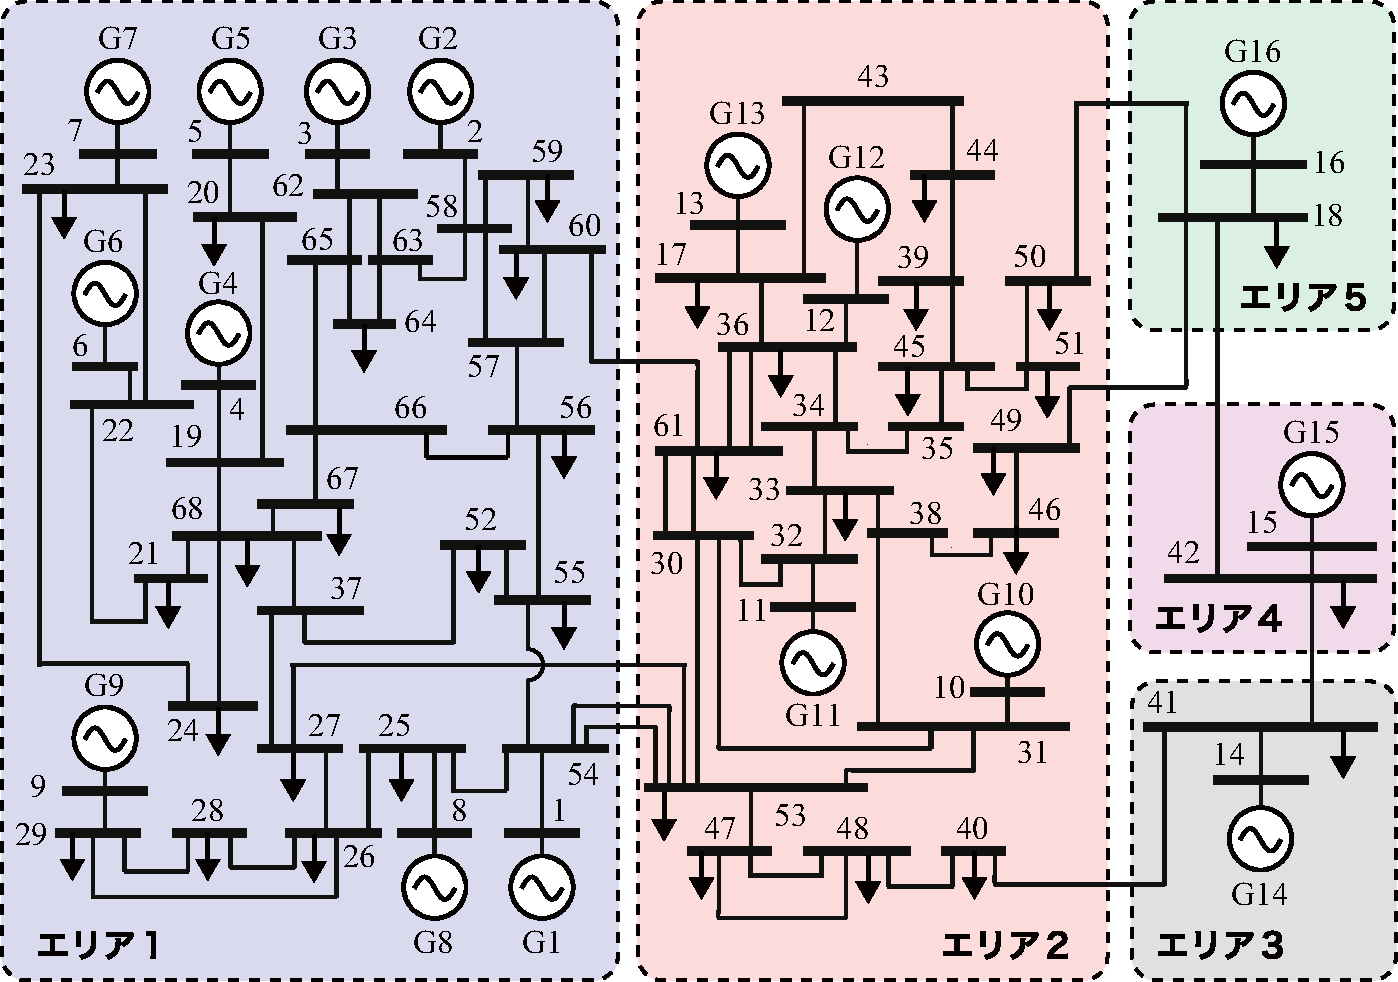
\includegraphics[width = .99\linewidth]{figs/IEEE68bus}
\medskip
\caption{\textbf{IEEE68母線系統モデル}}
\label{fig:IEEE68bus}
\medskip
\end{figure}

\subsection{IEEE68母線系統モデル}

本節では,IEEE68母線系統モデル(\FIGref{fig:IEEE68bus})を用いた数値シミュレーション結果を例示する。
このモデルは,68地点の母線で構成されており,そのうち16地点の母線に発電機,35地点の母線に負荷が接続されている。
\FIGref{fig:IEEE68bus}における「エリア1」は米国北東部のニューイングランド地域の電力系統を表しており,「エリア2」はニューヨーク州の電力系統を表している。
また,エリア3からエリア5は,ニューヨーク州周辺の電力系統をそれぞれ1組の発電機と負荷に集約して表現している。



送電線は,\ref{sec:transmodc}節で説明した対地静電容量を考慮したモデルとして設定する。
各送電線の定数は\TABref{table:ieee68lines}の値に設定する。
1列目は送電線端の母線番号,2列目,3列目,4列目はそれぞれ,送電線の抵抗,リアクタンス,対地静電容量の値を表す。
これらは\cite[Appendix A]{pal2006robust}に示されている標準的な値である。
また,発電機には\ref{sec:genmodadv}節で説明した突極型の発電機モデルを採用する。
各発電機の定数は\TABref{table:ieee68genpara}の値に設定する。
これらも上述の文献に示されている値である。



\subsection{潮流計算に用いるデータシート}


潮流計算に用いる発電機母線のデータシートを\TABref{table:ieee68datag}に示す。
同様に,負荷母線のデータシートを\TABref{table:ieee68datal}に示す。
これらも\cite[Appendix A]{pal2006robust}に示されている値を引用している。


\subsection{負荷モデル}

負荷モデルには\ref{sec:loadpr}節で説明した定インピーダンスモデルを採用する。
\TABref{table:ieee68datag}と\TABref{table:ieee68datal}のデータシートに対して,潮流計算の結果から定められる負荷のインピーダンス値は\TABref{table:ieee68loads}となる。
なお,母線16をスラック母線に設定しており,$P_{16}^{\star}$の値は33.68と求められる。





\section{負荷変動に対する周波数安定性解析}\label{sec:IEEE68AGC}

\subsection{負荷変動の設定}

本節では,負荷のインピーダンス値を変化させた場合の角周波数偏差の時間応答を観察する。
負荷のインピーダンスは,\TABref{table:ieee68loads}の値を基準として,1時間あたり10\%ずつ線形に増加させる。
すなわち,各負荷のインピーダンスは
\begin{align}\label{eq:loadvary68}
z_{{\rm load}i}(t) = \left(1+\tfrac{1}{36000}t \right) \left( r_{{\rm load}i} + \bm{j} x_{{\rm load}i} \right)
\end{align}
と設定する。
なお,時刻$t$の単位は[s]である。

\subsection{発電機の機械入力と界磁入力が定数である場合}\label{sec:constPV}

発電機の外部入力である機械入力と界磁入力がすべて定数である場合を考える。
\TABref{table:ieee68datag}と\TABref{table:ieee68datal}のデータシートに対する定常潮流状態から,式\ref{eq:loadvary68}にしたがって負荷のインピーダンスが変化した場合における,すべての発電機に関する角周波数偏差の時間応答を\FIGref{fig:omegasAGC}(a)に示す。
この場合には,負荷変動が生じると需給バランスが満たされないため,角周波数偏差は0にならないことがわかる。
また,負荷のインピーダンス値の増加に伴う消費電力の増加のため,はじめの約7秒間は角周波数偏差が負の方向に増大しており,その後は電力系統モデルが不安定となり正の方向に発散している。

\begin{figure}[t]
  \centering
  {
  \begin{minipage}{0.49\linewidth}
    \centering
    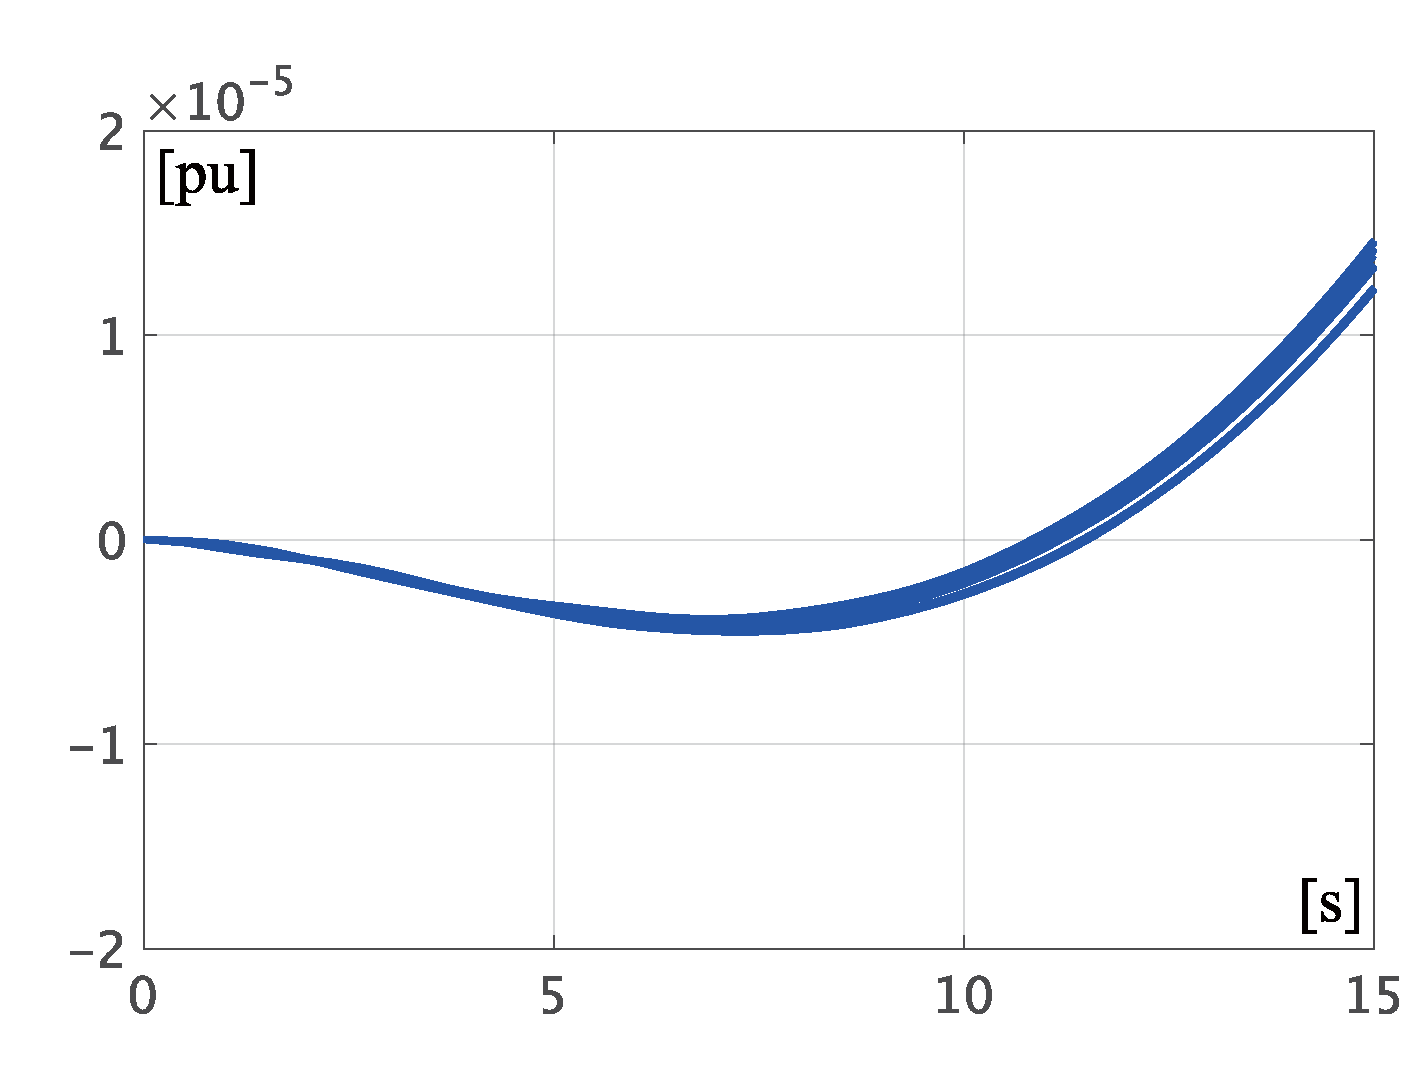
\includegraphics[width = 1.0\linewidth]{figs/WOavrWOagc}
    \subcaption{ 機械入力と界磁入力が定数の場合 }
    \medskip
  \end{minipage}
  \begin{minipage}{0.49\linewidth}
    \centering
    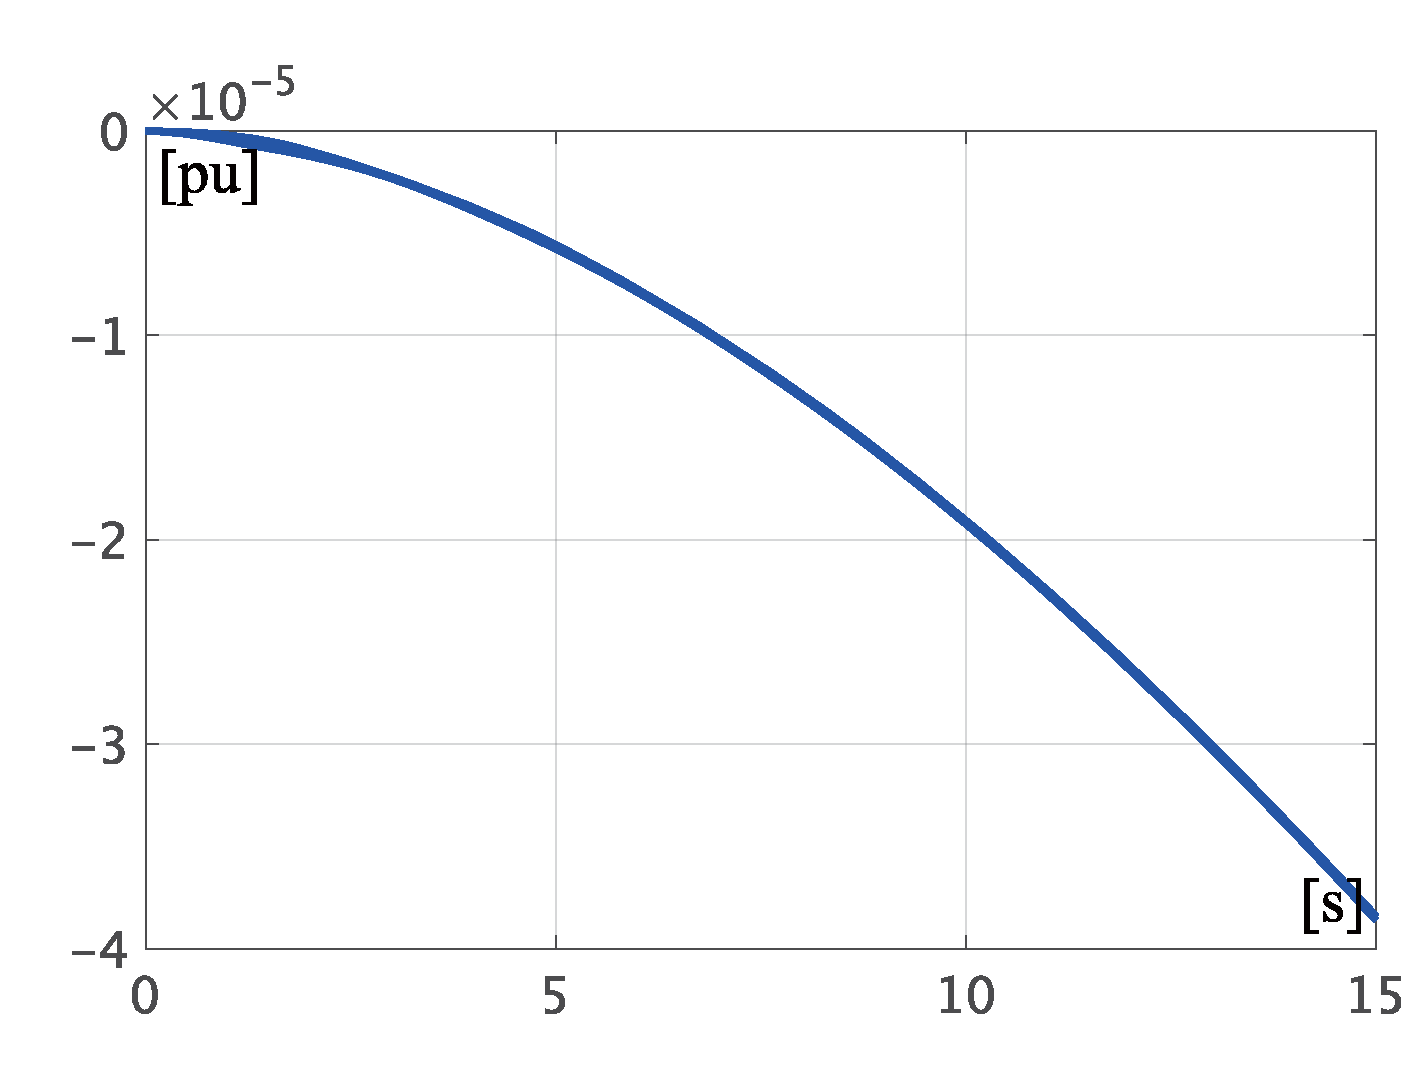
\includegraphics[width = 1.0\linewidth]{figs/WavrWOagc}
    \subcaption{ 機械入力が定数の場合 }
    \medskip
  \end{minipage}
 \begin{minipage}{0.49\linewidth}
    \centering
    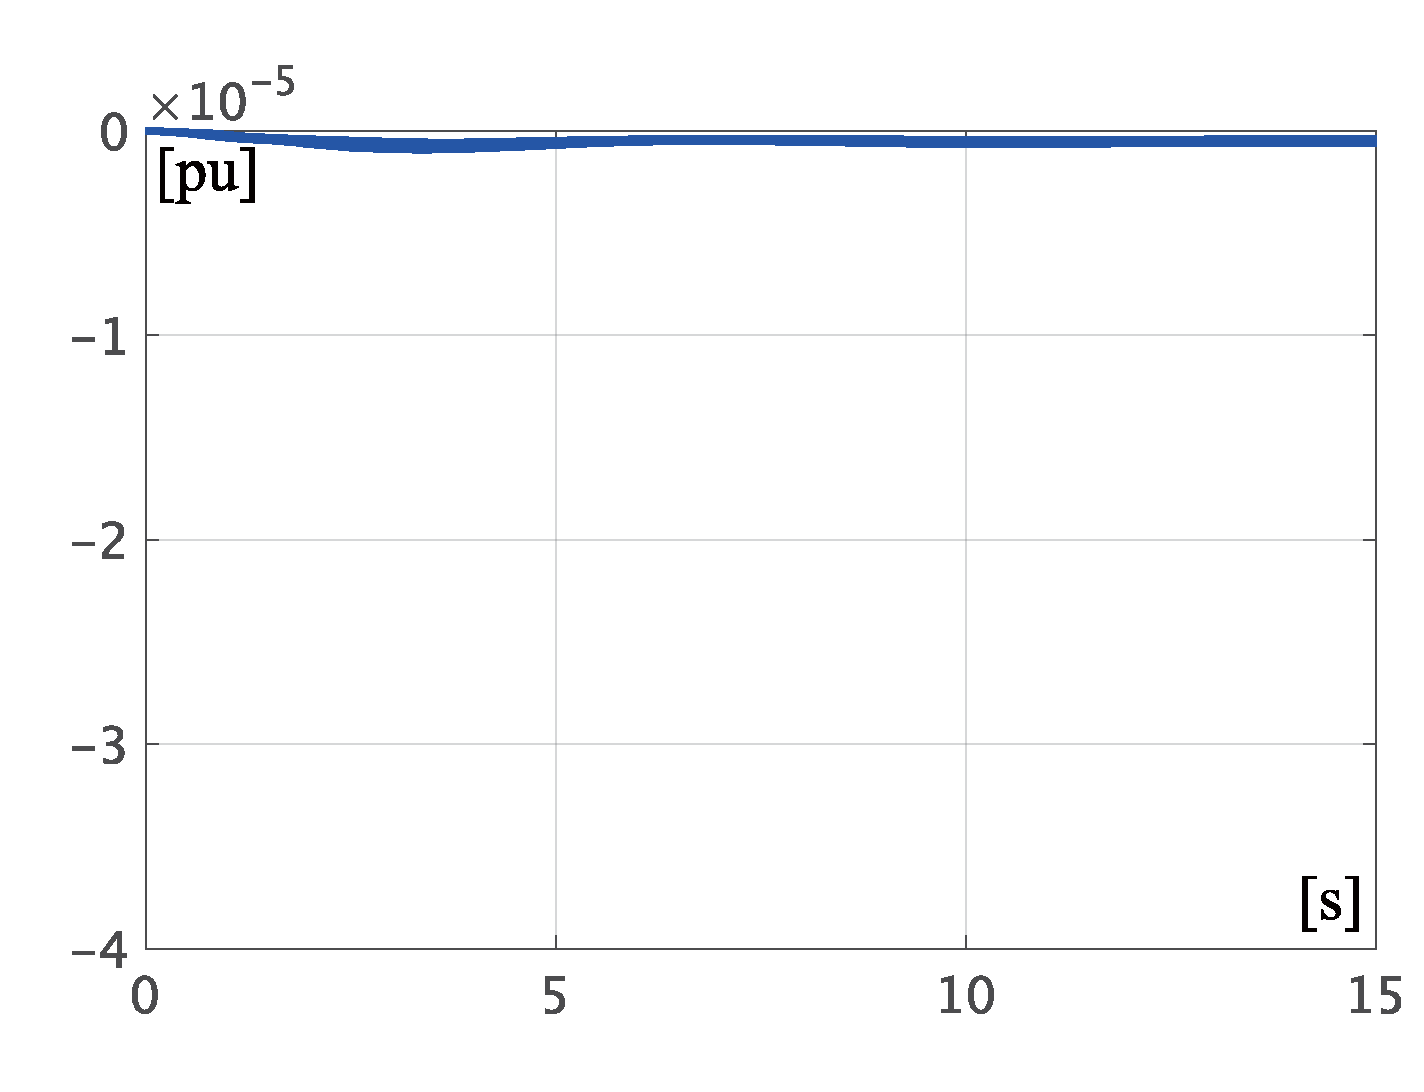
\includegraphics[width = 1.0\linewidth]{figs/WavrWagc}
    \subcaption{ 機械入力を制御する場合 }
    \medskip
  \end{minipage}
  \begin{minipage}{0.49\linewidth}
    \centering
    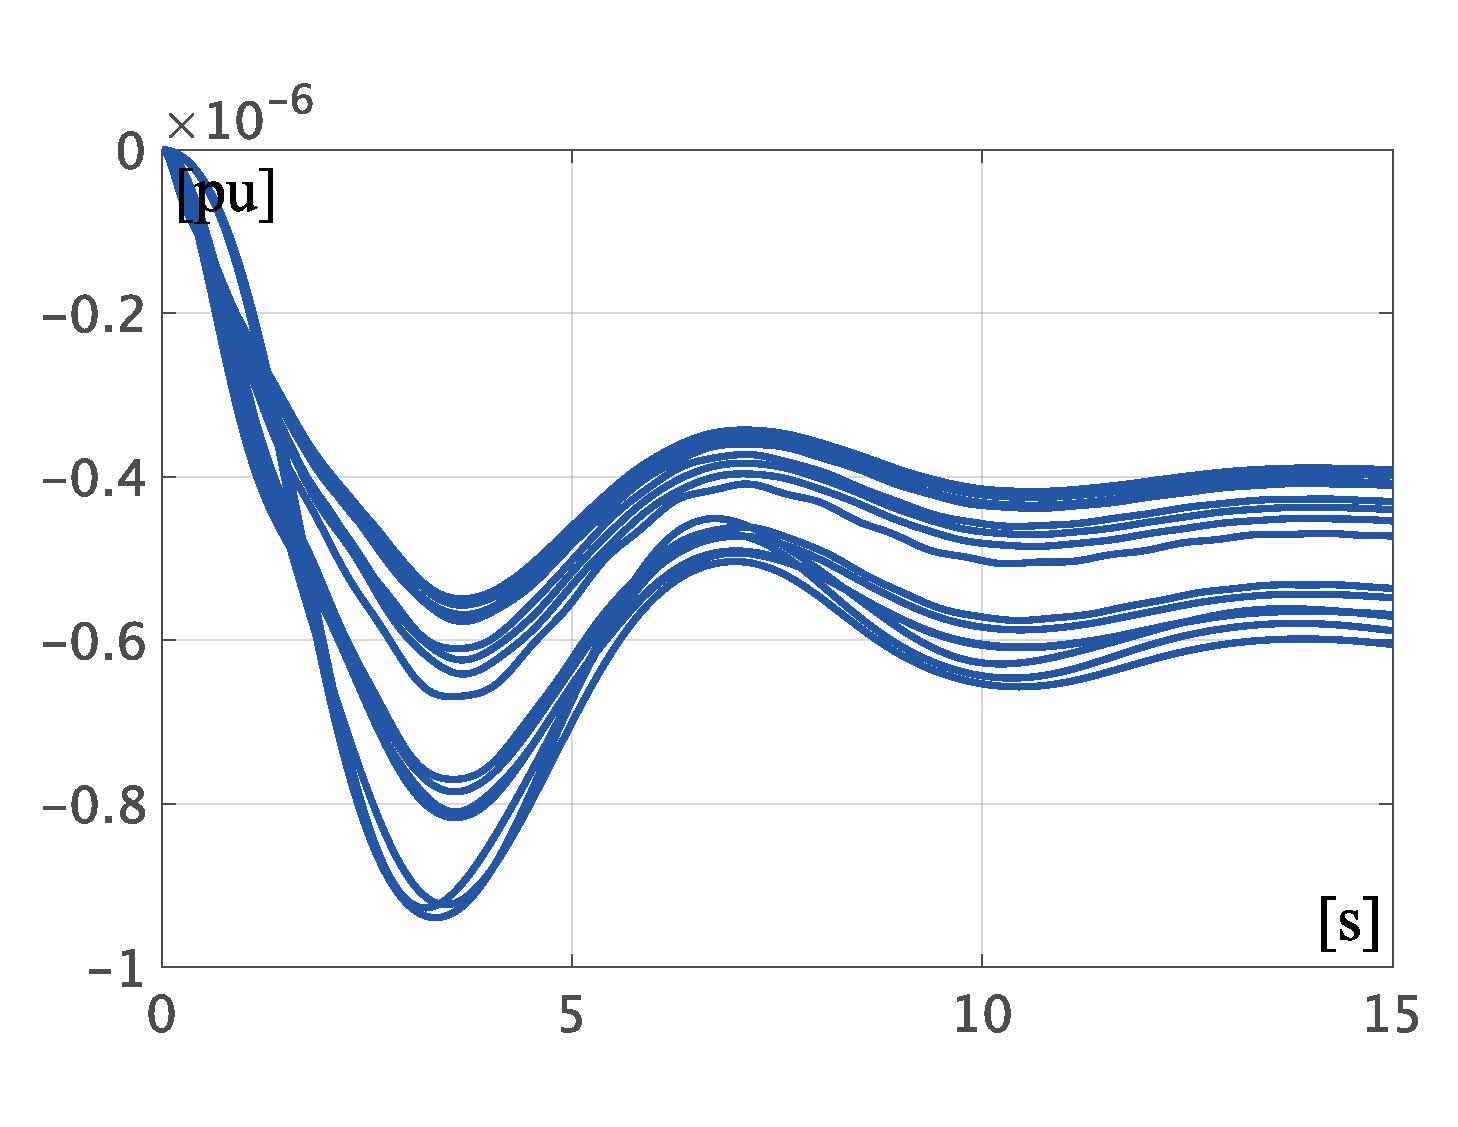
\includegraphics[width = 1.0\linewidth]{figs/WavrWagcL}
    \subcaption{ 機械入力を制御する場合(拡大) }
    \medskip
  \end{minipage}
  }
  \medskip
  \caption{\textbf{負荷変動に対する角周波数偏差の時間応答} }
  \label{fig:omegasAGC}
\medskip
\end{figure}

\subsection{機械入力が定数である場合}\label{sec:onlyAVR}

発電機の界磁入力を制御する自動電圧調整器と系統安定化装置が,各々すべての発電機に組み込まれた場合を考える。
自動電圧調整器は\ref{sec:avrov}節のIEEE ST1型モデルに設定する。
具体的には,すべての発電機母線$i$に対して
\begin{align*}
\simode{
0.015 \dot{V}_{{\rm tr}i} & = - V_{{\rm tr} i} +  |\bm{V}_i|  \\
V_{{\rm field}i} &= 20 ( V_{{\rm ref}i}^{\star} + V_{{\rm pss}i}- V_{{\rm tr}i} )
}
\end{align*}
に設定する。
また,系統安定化装置は\ref{sec:pssintro}節のIEEE PSS1 型モデルとする。
具体的には,すべての発電機母線$i$に対して
\begin{align*}
\simode{
1.4 \dot{\xi}_{{\rm ws}i} &=
- \xi_{{\rm ws}i}
+ 9.5 \Delta \omega_i \\
v_{{\rm ws}i} &= 9.5 \Delta \omega_i - \xi_{{\rm ws}i}
}
\qquad
\simode{
0.033 \dot{\xi}_{i} &=
- \xi_{i}
+ 0.79 
v_{{\rm ws}i} \\
V_{{\rm pss}i} &= 4.67 ( v_{{\rm ws}i} - \xi_{i} )
}
\end{align*}
に設定する。
この場合の角周波数偏差の時間応答を\FIGref{fig:omegasAGC}(b)に示す。
\FIGref{fig:omegasAGC}(a)と同様に,負荷変動のため需給バランスが満たされず,角周波数偏差は0にならないことがわかる。
なお,発電機の機械入力は,\ref{sec:constPV}節と同様にすべて定数としている。




\subsection{自動発電制御器により機械入力を制御する場合}

発電機の機械入力を制御する自動発電制御器を組み込む場合を考える。
ここでは,\FIGref{fig:IEEE68bus}の各々すべてのエリアに対して,\ref{sec:broadPI}節で説明したブロードキャスト型PIコントローラを組み込む。
具体的には,エリア$l$に属する発電機母線の添字集合を$\mathcal{I}^{(l)}_{\rm G}$と表して,エリア$l$の自動発電制御器を
\begin{align*}
\simode{
\dot{\xi}^{(l)}&=  \Delta \omega_{\rm ave}^{(l)}\\
P_{{\rm mech}i} &= P_{i}^{\star} 
- \tfrac{ P_{i}^{\star} }{ P_{{\rm ave}}^{{\star}} } \left(  100 \Delta \omega_{\rm ave}^{(l)} +  500  \xi^{(l)} \right),
\qquad i \in \mathcal{I}^{(l)}_{\rm G}
}
\end{align*}
に設定する。
ただし,エリア$l$に属する発電機の角周波数偏差の平均値と定常状態における有効電力の平均値を
\[
\Delta \omega_{\rm ave}^{(l)}(t) := 
\frac{ 1 }{|\mathcal{I}^{(l)}_{\rm G}|}
\sum_{i \in \mathcal{I}^{(l)}_{\rm G}}  \Delta \omega_{i}(t)
,\qquad
P_{{\rm ave}}^{{\star}} := 
\frac{ 1 }{ 16 }
\sum_{i =1}^{16}  P_{i}^{\star}
\]
と定義している。
なお,自動電圧調整器は,\ref{sec:onlyAVR}節と同じものが各発電機に組み込まれているものとする。

この場合の角周波数偏差の時間応答を\FIGref{fig:omegasAGC}(c)に示す。
なお,\FIGref{fig:omegasAGC}(d)は縦軸のスケールを拡大したものである。
自動発電制御の働きによって,角周波数偏差は0付近の値に維持されていることがわかる。
なお,負荷のインピーダンス値が継続して変化しているため角周波数偏差は厳密に0にはならないが,$-1\times 10^{-6}$~[pu]程度の小さな値となっていることもわかる。

\begin{figure}[t!]
  \centering
  {
  \begin{minipage}{0.49\linewidth}
    \centering
    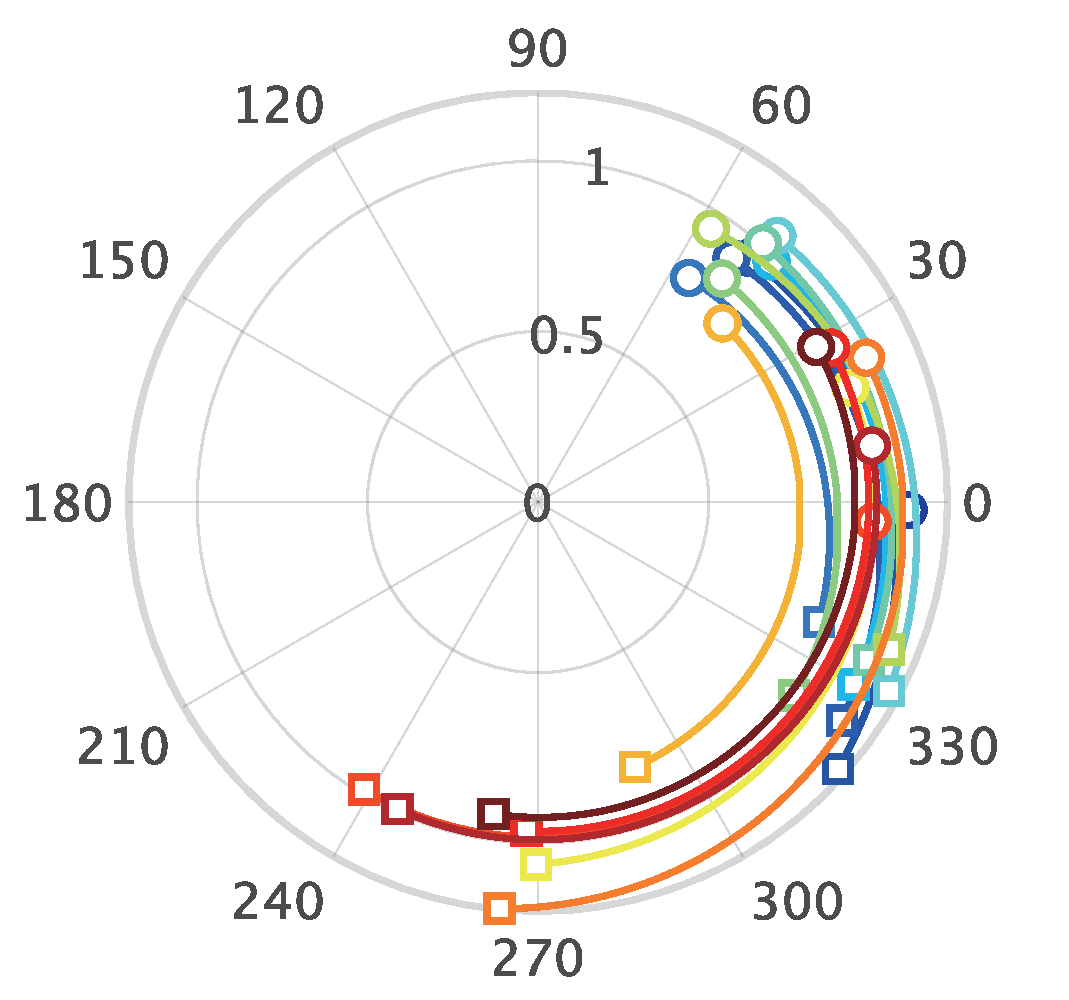
\includegraphics[width = 0.9\linewidth]{figs/Epolar}
    \subcaption{ $E_i e^{\bm{j} \delta_i}$~[pu]}
    \medskip
  \end{minipage}
  \begin{minipage}{0.49\linewidth}
    \centering
    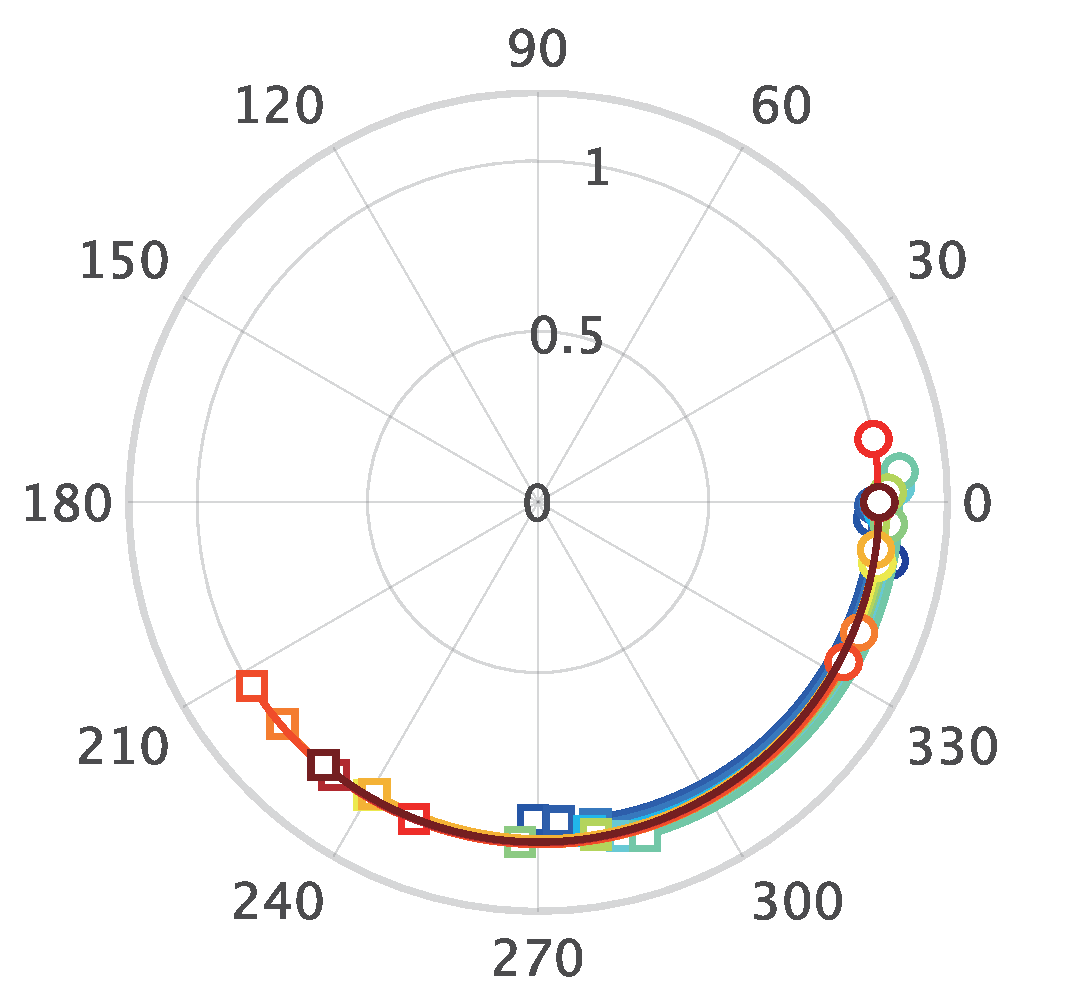
\includegraphics[width = 0.9\linewidth]{figs/Vpolar}
    \subcaption{ $\bm{V}_i$~[pu] }
    \medskip
  \end{minipage}
 \begin{minipage}{0.49\linewidth}
    \centering
    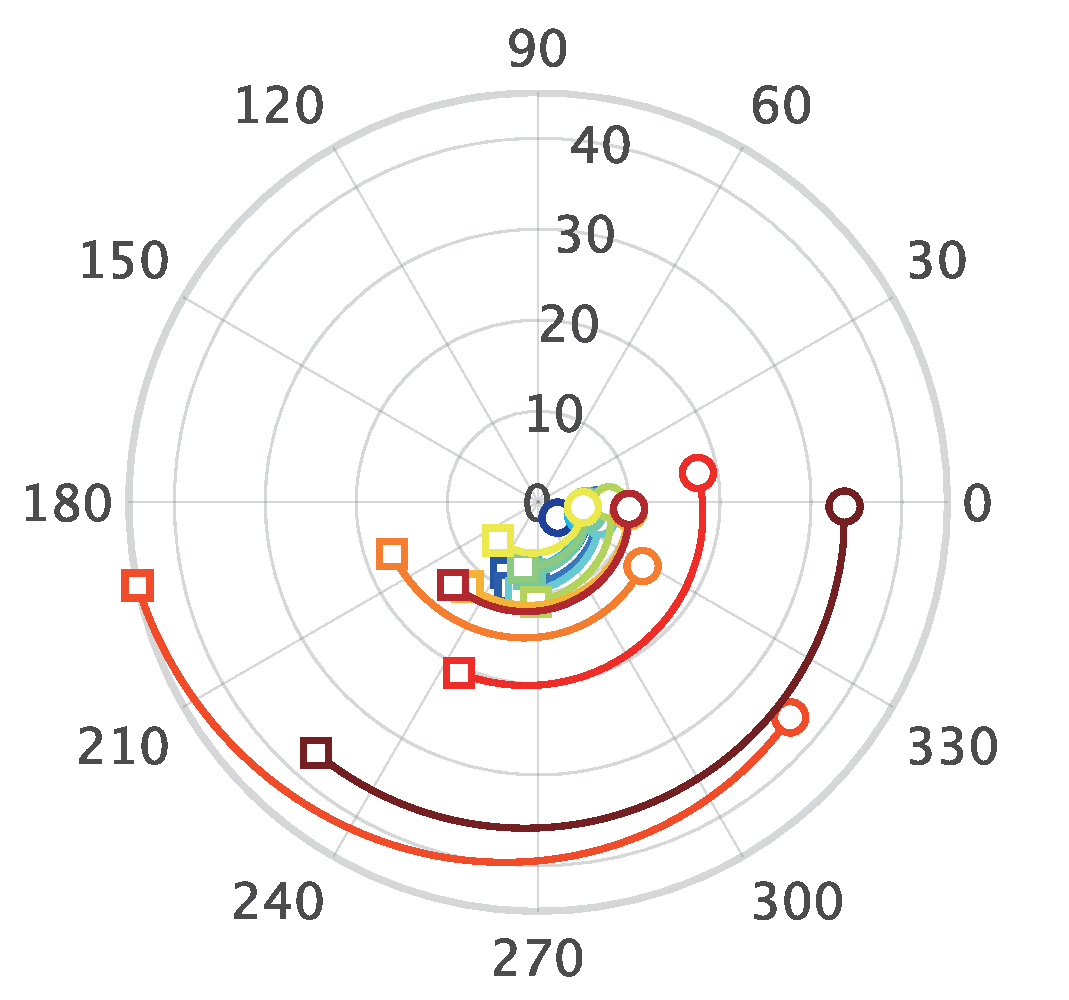
\includegraphics[width = 0.9\linewidth]{figs/Ipolar}
    \subcaption{ $\bm{I}_i$~[pu] }
    \medskip
  \end{minipage}
  \begin{minipage}{0.49\linewidth}
    \centering
    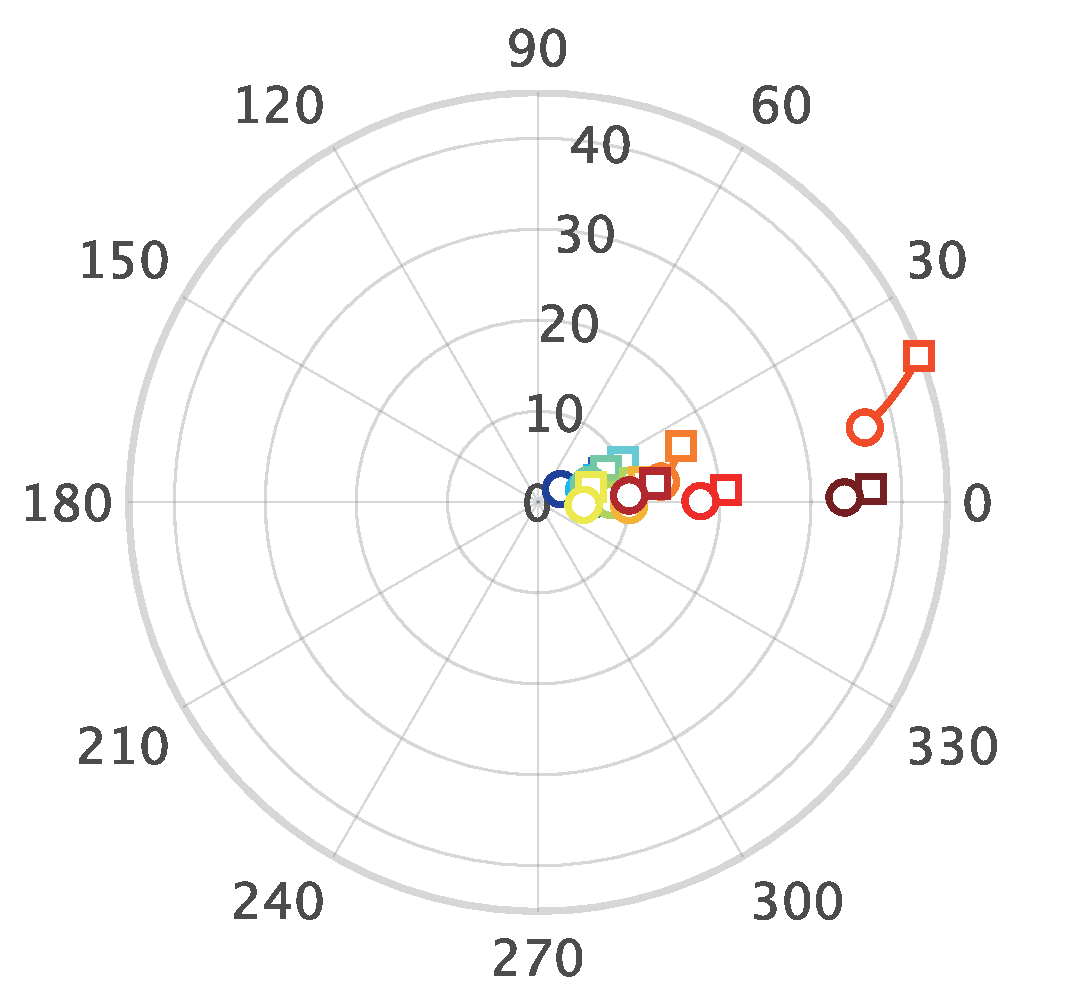
\includegraphics[width = 0.9\linewidth]{figs/PQpolar}
    \subcaption{ $P+\bm{j}Q$~[pu] }
    \medskip
  \end{minipage}
  }
  \medskip
  \caption{\textbf{負荷変動に対する発電機変数と母線変数の変化}
  \\  \centering(丸:初期時刻,四角:終端時刻)}
  \label{fig:polars}
\medskip
\end{figure}


つぎに,初期時刻から3時間が経過するまでの発電機変数と母線変数の変化を\FIGref{fig:polars}に示す。
\FIGref{fig:polars}(a)--(d)はそれぞれ,$E_i e^{\bm{j} \delta_i}$,$\bm{V}_i$,$\bm{I}_i$,$P_i+\bm{j}Q_i$の変化を複素平面上に極座標表示したものである。
初期時刻$t=0$における値を丸の印,終端時刻$t=10800$における値を四角の印で表示している。
この図から以下のことが読み取れる。

\begin{itemize}
\item \FIGref{fig:polars}(a):すべての発電機の内部電圧は0.7から1.5~[pu]程度の大きさに維持されており,回転子偏角は時計回りに緩やかに変化している。
\item \FIGref{fig:polars}(b):母線電圧の絶対値は1~[pu]付近で維持されており,位相は回転子偏角と同様に時計回りに緩やかに変化している。
\item \FIGref{fig:polars}(c):負荷のインピーダンス値の増加に伴う消費電力の増加に合わせて,母線電流の絶対値が増加している。
\item \FIGref{fig:polars}(d):負荷のインピーダンス値の増加に合わせて,母線に供給される有効電力と無効電力が増加している。
\end{itemize}

以上の結果から,自動発電制御によって周波数の安定化が適切に実現されていることがわかる。
また,緩やかな負荷変動に対しては,発電機の内部状態も振動することなく緩やかに変化すること,すなわち,電力系統全体が準定常状態にあることがわかる。




\section{母線地絡に対する過渡安定度解析}\label{sec:IEEE68PSS}

\subsection{母線地絡の設定}

本節では,母線地絡に対する過渡安定度の解析を行う。
電力系統の過渡安定度は以下のように評価する。
母線$k$における地絡によって生じる発電機$i$の角周波数偏差を$\Delta \omega_i^{(k)}$と表す。
このとき,母線$k$の地絡に対する電力系統全体の角周波数偏差の感度を$\|\Delta \omega^{(k)}\|_{\mathcal{L}_2}$により評価する。
ただし,$\Delta \omega^{(k)}$はすべての発電機の角周波数偏差$\Delta \omega_1^{(k)},\ldots,\Delta \omega_{16}^{(k)}$を並べたベクトルである。
また,すべての発電機母線と負荷母線に関して$\|\Delta \omega^{(k)}\|_{\mathcal{L}_2}$の値を並べた集合をそれぞれ
\begin{align*}%\label{eq:JGJL}
\mathcal{J}_{\rm G}:=
\left\{
\| \Delta \omega^{(k)} \|_{\mathcal{L}_2}
\right\}_{k\in \{1,\ldots,16\} }
,\qquad
\mathcal{J}_{\rm L}
:=
\left\{
\| \Delta \omega^{(k)} \|_{\mathcal{L}_2}
\right\}_{k\in \{17,\ldots,68\} }
\end{align*}
と定義する。
地絡は特定の母線のみではなく,すべての母線に生じる可能性があることを考慮すると,母線地絡に対する過渡安定度の高さは,データ集合$\mathcal{J}_{\rm G}$と$\mathcal{J}_{\rm L}$が適切な意味で小さいこととして評価できる。
本節では,データのばらつきの大きさを可視化するために,$\mathcal{J}_{\rm G}$と$\mathcal{J}_{\rm L}$を箱ひげ図で表示することにより,それらの最大値,最小値,四分位数を用いて過渡安定度の比較に用いる。
なお,地絡の継続時間はすべて70~[ms]に設定する。

\begin{figure}[t!]
  \centering
  {
  \begin{minipage}{0.49\linewidth}
    \centering
    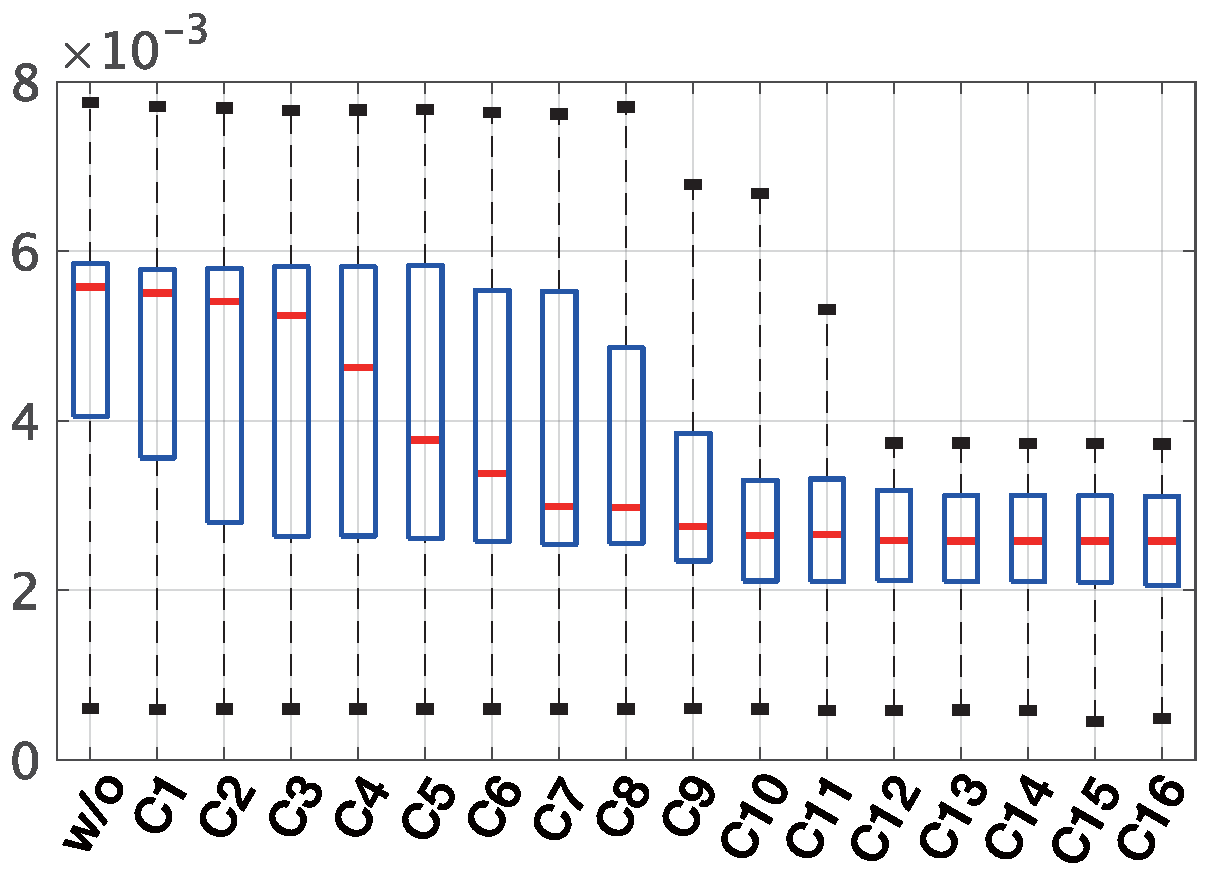
\includegraphics[width = 1.0\linewidth]{figs/boxplotgen}
    \subcaption{ $\mathcal{J}_{\rm G}$:発電機母線の地絡}
  \end{minipage}
  \begin{minipage}{0.49\linewidth}
    \centering
    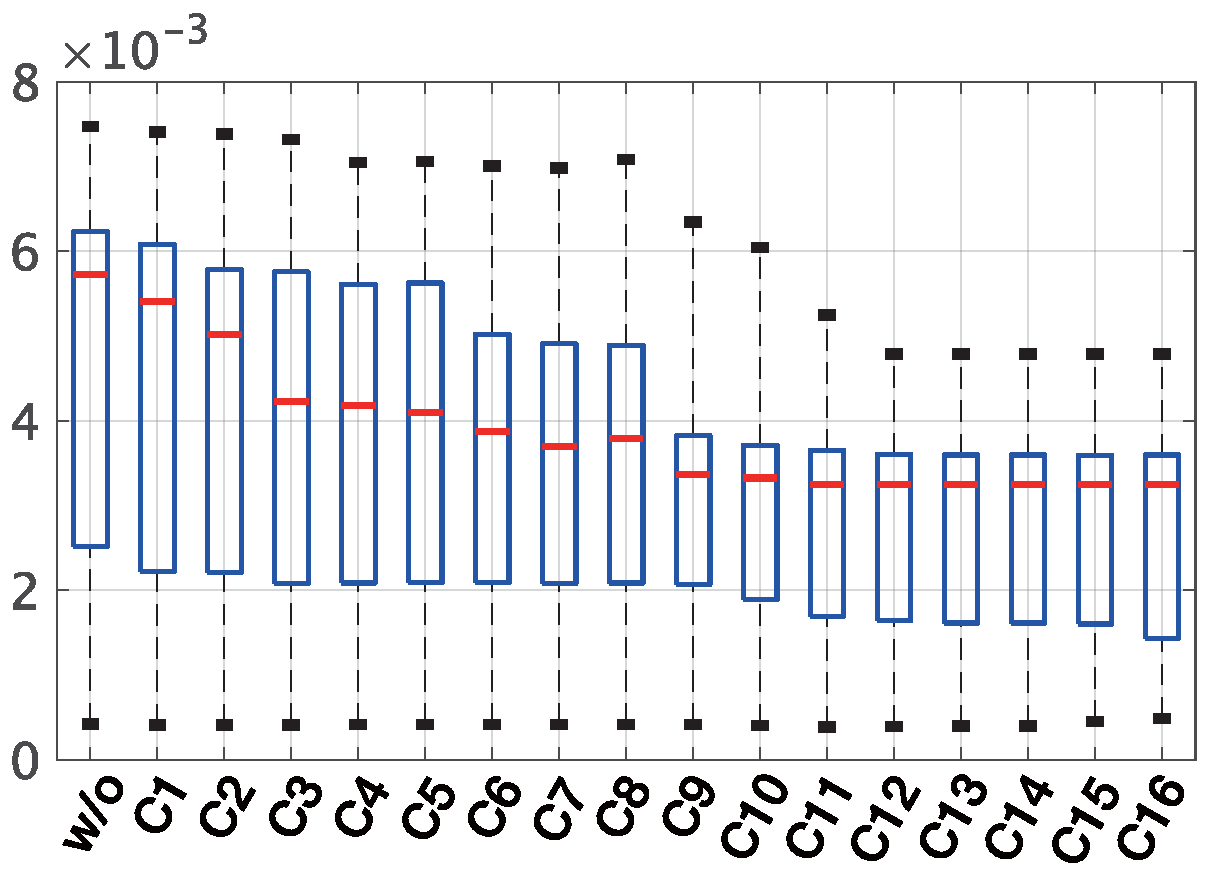
\includegraphics[width = 1.0\linewidth]{figs/boxplotload}
    \subcaption{ $\mathcal{J}_{\rm L}$:負荷母線の地絡}
  \end{minipage}
  \medskip
  \caption{\textbf{母線地絡に対する系統安定度の評価} }
  \label{fig:boxplots}
  }
\medskip
\end{figure}

まず,すべての発電機に標準的な自動電圧調整器と系統安定化装置が組み込まれている場合の過渡安定度を解析する。
パラメータの設定は,\ref{sec:onlyAVR}節と同様であるものとする。
得られたデータ集合$\mathcal{J}_{\rm G}$と$\mathcal{J}_{\rm L}$を箱ひげ図として表示した結果を\FIGref{fig:boxplots}の1列目に示す。
\FIGref{fig:boxplots}(a)が発電機母線の地絡に関する$\mathcal{J}_{\rm G}$であり,\FIGref{fig:boxplots}(b)が負荷母線の地絡に関する$\mathcal{J}_{\rm L}$である。
以下では,これらの値を基準として,局所的なコントローラの追加による過渡安定度の向上を評価する。

\subsection{レトロフィット制御理論に基づく系統安定化装置の効果}

\ref{sec:retrofit}節で説明したレトロフィット制御理論に基づく系統安定化装置が各発電機に組み込まれた場合の過渡安定度を解析する。
各発電機に組み込まれるレトロフィットコントローラには,例\ref{ex:modelingV}の手順によって計測データから同定された近似線形環境モデルのパラメータを用いる。
なお,局所線形サブシステム$G_i$には,自動電圧調整器に加えて系統安定化装置のモデルも用いる。
また,個々の設計用モデル$G^+_i$を安定化するコントローラは,\ref{sec:designret}節で説明された線形2次レギュレータの設計手法に基づいて設計する。

このとき,得られたデータ集合$\mathcal{J}_{\rm G}$と$\mathcal{J}_{\rm L}$を箱ひげ図として表示した結果を\FIGref{fig:boxplots}の2列目から17列目に示す。
横軸の「C$i$」は,発電機1から発電機$i$の各々すべてにレトロフィットコントローラが組み込まれた場合を表している。
この結果から,組み込まれるレトロフィットコントローラの数が増加することにより,系統安定度が段階的に向上していることがわかる。



\begin{table}[h]
\medskip
\caption{\textbf{送電線の物理定数}} \label{table:ieee68lines}
 \centering
  {
  \begin{minipage}{0.49\linewidth}
    \centering
  \begin{tabular}{crrrrcc}
   \hline
$i$--$j$ & $r_{ij}$  &  $x_{ij}$ & $c_{ij}$ \\
   \hline \hline
1--54  & 0 & 0.0181 & 0 \\
2--58  & 0 & 0.0250 & 0 \\
3--62  & 0 & 0.0200 & 0 \\
4--19  & 0.0007 & 0.0142 & 0 \\
5--20  & 0.0009 & 0.0180 & 0 \\
6--22  & 0 & 0.0143 & 0 \\
7--23  & 0.0005 & 0.0272 & 0 \\
8--25  & 0.0006 & 0.0232 & 0 \\
9--29  & 0.0008 & 0.0156 & 0 \\
10--31  & 0 & 0.0260 & 0 \\
11--32  & 0 & 0.0130 & 0 \\
12--36  & 0 & 0.0075 & 0 \\
13--17  & 0 & 0.0033 & 0 \\
14--41  & 0 & 0.0015 & 0 \\
15--42  & 0 & 0.0015 & 0 \\
16--18  & 0 & 0.0030 & 0 \\
17--36  & 0.0005 & 0.0045 & 0.3200 \\
17--43  & 0.0005 & 0.0276 & 0 \\
18--42  & 0.0040 & 0.0600 & 2.2500 \\
18--49  & 0.0076 & 0.1141 & 1.1600 \\
19--20  & 0.0007 & 0.0138 & 0 \\
19--68  & 0.0016 & 0.0195 & 0.3040 \\
21--22  & 0.0008 & 0.0140 & 0.2565 \\
21--68  & 0.0008 & 0.0135 & 0.2548 \\
22--23  & 0.0006 & 0.0096 & 0.1846 \\
23--24  & 0.0022 & 0.0350 & 0.3610 \\
24--68  & 0.0003 & 0.0059 & 0.0680 \\
25--26  & 0.0032 & 0.0323 & 0.5310 \\
25--54  & 0.0070 & 0.0086 & 0.1460 \\
26--27  & 0.0014 & 0.0147 & 0.2396 \\
26--28  & 0.0043 & 0.0474 & 0.7802 \\
26--29  & 0.0057 & 0.0625 & 1.0290 \\
27--37  & 0.0013 & 0.0173 & 0.3216 \\
27--53  & 0.0320 & 0.3200 & 0.4100 \\
28--29  & 0.0014 & 0.0151 & 0.2490 \\
30--31  & 0.0013 & 0.0187 & 0.3330 \\
30--32  & 0.0024 & 0.0288 & 0.4880 \\
30--53  & 0.0008 & 0.0074 & 0.4800 \\
30--61  & 0.0019 & 0.0183 & 0.2900 \\
30--61  & 0.0019 & 0.0183 & 0.2900 \\
31--38  & 0.0011 & 0.0147 & 0.2470 \\
31--53  & 0.0016 & 0.0163 & 0.2500 \\
32--33  & 0.0008 & 0.0099 & 0.1680 \\
\hline
  \end{tabular}
%  \subcaption{データシート}
  \end{minipage}
  \begin{minipage}{0.49\linewidth}
    \centering
  \begin{tabular}{crrrcc}
   \hline
$i$--$j$ & $r_{ij}$  &  $x_{ij}$ & $c_{ij}$ \\
   \hline \hline
33--34  & 0.0011 & 0.0157 & 0.2020 \\
33--38  & 0.0036 & 0.0444 & 0.6930 \\
34--35  & 0.0001 & 0.0074 & 0 \\
34--36  & 0.0033 & 0.0111 & 1.4500 \\
35--45  & 0.0007 & 0.0175 & 1.3900 \\
36--61  & 0.0022 & 0.0196 & 0.3400 \\
36--61  & 0.0022 & 0.0196 & 0.3400 \\
37--52  & 0.0007 & 0.0082 & 0.1319 \\
37--68  & 0.0007 & 0.0089 & 0.1342 \\
38--46  & 0.0022 & 0.0284 & 0.4300 \\
39--44  & 0 & 0.0411 & 0 \\
39--45  & 0 & 0.0839 & 0 \\
40--41  & 0.0060 & 0.0840 & 3.1500 \\
40--48  & 0.0020 & 0.0220 & 1.2800 \\
41--42  & 0.0040 & 0.0600 & 2.2500 \\
43--44  & 0.0001 & 0.0011 & 0 \\
44--45  & 0.0025 & 0.0730 & 0 \\
45--51  & 0.0004 & 0.0105 & 0.7200 \\
46--49  & 0.0018 & 0.0274 & 0.2700 \\
47--48  & 0.0025 & 0.0268 & 0.4000 \\
47--48  & 0.0025 & 0.0268 & 0.4000 \\
47--53  & 0.0013 & 0.0188 & 1.3100 \\
50--51  & 0.0009 & 0.0221 & 1.6200 \\
52--55  & 0.0011 & 0.0133 & 0.2138 \\
53--54  & 0.0035 & 0.0411 & 0.6987 \\
54--55  & 0.0013 & 0.0151 & 0.2572 \\
55--56  & 0.0013 & 0.0213 & 0.2214 \\
56--57  & 0.0008 & 0.0128 & 0.1342 \\
56--66  & 0.0008 & 0.0129 & 0.1382 \\
57--58  & 0.0002 & 0.0026 & 0.0434 \\
58--59  & 0.0006 & 0.0092 & 0.1130 \\
57--60  & 0.0008 & 0.0112 & 0.1476 \\
59--60  & 0.0004 & 0.0046 & 0.0780 \\
60--61  & 0.0023 & 0.0363 & 0.3804 \\
58--63  & 0.0007 & 0.0082 & 0.1389 \\
62--63  & 0.0004 & 0.0043 & 0.0729 \\
62--65  & 0.0004 & 0.0043 & 0.0729 \\
63--64  & 0.0016 & 0.0435 & 0 \\
64--65  & 0.0016 & 0.0435 & 0 \\
65--66  & 0.0009 & 0.0101 & 0.1723 \\
66--67  & 0.0018 & 0.0217 & 0.3660 \\
67--68  & 0.0009 & 0.0094 & 0.1710 \\
\\
   \hline
  \end{tabular}
%   \subcaption{潮流計算結果}
  \end{minipage}
  }
\end{table}


\begin{table}[h]
\medskip
\caption{\textbf{発電機の物理定数}} \label{table:ieee68genpara}
 \centering
 {
\begin{tabular}{crrrrrr}
   \hline
\multicolumn{1}{c}{$i$} & \multicolumn{1}{r}{$M_{i}$} & \multicolumn{1}{r}{$D_{i}$} & \multicolumn{1}{r}{$\tau_{i}$} & \multicolumn{1}{r}{$X_{{\rm d}i}$} & \multicolumn{1}{r}{$X_{{\rm q}i}$} & \multicolumn{1}{r}{$X_{{\rm d}i}'$}  \\
   \hline \hline
1  & \multicolumn{1}{r}{42.0}  & \multicolumn{1}{r}{4.00} & \multicolumn{1}{r}{10.20} & \multicolumn{1}{r}{0.100} & \multicolumn{1}{r}{0.069} & \multicolumn{1}{r}{0.031} \\
2  & \multicolumn{1}{r}{30.2}  & \multicolumn{1}{r}{9.75} & \multicolumn{1}{r}{6.56} & \multicolumn{1}{r}{0.295} & \multicolumn{1}{r}{0.282} & \multicolumn{1}{r}{0.070} \\
3  & \multicolumn{1}{r}{35.8}  & \multicolumn{1}{r}{10.00} & \multicolumn{1}{r}{5.70} & \multicolumn{1}{r}{0.250} & \multicolumn{1}{r}{0.237} & \multicolumn{1}{r}{0.053} \\
4  & \multicolumn{1}{r}{28.6}  & \multicolumn{1}{r}{10.00} & \multicolumn{1}{r}{5.69} & \multicolumn{1}{r}{0.262} & \multicolumn{1}{r}{0.258} & \multicolumn{1}{r}{0.044} \\
5  & \multicolumn{1}{r}{26.0}  & \multicolumn{1}{r}{3.00} & \multicolumn{1}{r}{5.40} & \multicolumn{1}{r}{0.330} & \multicolumn{1}{r}{0.310} & \multicolumn{1}{r}{0.066} \\
6  & \multicolumn{1}{r}{34.8}  & \multicolumn{1}{r}{10.00} & \multicolumn{1}{r}{7.30} & \multicolumn{1}{r}{0.254} & \multicolumn{1}{r}{0.241} & \multicolumn{1}{r}{0.050} \\
7  & \multicolumn{1}{r}{26.4}  & \multicolumn{1}{r}{8.00} & \multicolumn{1}{r}{5.66} & \multicolumn{1}{r}{0.295} & \multicolumn{1}{r}{0.292} & \multicolumn{1}{r}{0.049} \\
8  & \multicolumn{1}{r}{24.3}  & \multicolumn{1}{r}{9.00} & \multicolumn{1}{r}{6.70} & \multicolumn{1}{r}{0.290} & \multicolumn{1}{r}{0.280} & \multicolumn{1}{r}{0.057} \\
9  & \multicolumn{1}{r}{34.5}  & \multicolumn{1}{r}{14.00} & \multicolumn{1}{r}{4.79} & \multicolumn{1}{r}{0.211} & \multicolumn{1}{r}{0.205} & \multicolumn{1}{r}{0.057} \\
10 & \multicolumn{1}{r}{31.0}  & \multicolumn{1}{r}{5.56} & \multicolumn{1}{r}{9.37} & \multicolumn{1}{r}{0.169} & \multicolumn{1}{r}{0.115} & \multicolumn{1}{r}{0.046} \\
11 & \multicolumn{1}{r}{28.2}  & \multicolumn{1}{r}{13.60} & \multicolumn{1}{r}{4.10} & \multicolumn{1}{r}{0.128} & \multicolumn{1}{r}{0.123} & \multicolumn{1}{r}{0.018} \\
12 & \multicolumn{1}{r}{92.3}  & \multicolumn{1}{r}{13.50} & \multicolumn{1}{r}{7.40} & \multicolumn{1}{r}{0.101} & \multicolumn{1}{r}{0.095} & \multicolumn{1}{r}{0.031} \\
13 & \multicolumn{1}{r}{248.0}  & \multicolumn{1}{r}{33.00} & \multicolumn{1}{r}{5.90} & \multicolumn{1}{r}{0.030} & \multicolumn{1}{r}{0.029} & \multicolumn{1}{r}{0.006} \\
14 & \multicolumn{1}{r}{300.0}  & \multicolumn{1}{r}{100.00} & \multicolumn{1}{r}{4.10} & \multicolumn{1}{r}{0.018} & \multicolumn{1}{r}{0.017} & \multicolumn{1}{r}{0.003} \\
15 & \multicolumn{1}{r}{300.0}  & \multicolumn{1}{r}{100.00} & \multicolumn{1}{r}{4.10} & \multicolumn{1}{r}{0.018} & \multicolumn{1}{r}{0.017} & \multicolumn{1}{r}{0.003} \\
16 & \multicolumn{1}{r}{225.0}  & \multicolumn{1}{r}{50.00} & \multicolumn{1}{r}{7.80} & \multicolumn{1}{r}{0.036} & \multicolumn{1}{r}{0.033} & \multicolumn{1}{r}{0.007} \\
\hline
\end{tabular}
}
\end{table}





\begin{table}[h]
\medskip
\caption{\textbf{潮流計算に用いるデータシート(発電機母線)}} \label{table:ieee68datag}
 \centering
  {
  \begin{minipage}{0.32\linewidth}
    \centering
  \begin{tabular}{crrcc}
   \hline
$i$ & $P_i^{\star}$  &  $|\bm{V}_i^{\star} |$ \\
   \hline \hline
1  & \multicolumn{1}{r}{2.50}   & \multicolumn{1}{r}{1.045} \\
2  & \multicolumn{1}{r}{5.45}   & \multicolumn{1}{r}{0.980} \\
3  & \multicolumn{1}{r}{6.50}   & \multicolumn{1}{r}{0.983} \\
4  & \multicolumn{1}{r}{6.32}   & \multicolumn{1}{r}{0.997} \\
5  & \multicolumn{1}{r}{5.05}   & \multicolumn{1}{r}{1.011} \\
6  & \multicolumn{1}{r}{7.00}   & \multicolumn{1}{r}{1.050} \\
   \hline
  \end{tabular}
%  \subcaption{データシート}
  \end{minipage}
  \begin{minipage}{0.32\linewidth}
    \centering
  \begin{tabular}{ccccc}
   \hline
$i$ & $P_i^{\star}$  &  $|\bm{V}_i^{\star} |$ \\
   \hline \hline
7  & \multicolumn{1}{r}{5.60}   & \multicolumn{1}{r}{1.063} \\
8  & \multicolumn{1}{r}{5.40}   & \multicolumn{1}{r}{1.030} \\
9  & \multicolumn{1}{r}{8.00}   & \multicolumn{1}{r}{1.025} \\
10 & \multicolumn{1}{r}{5.00}   & \multicolumn{1}{r}{1.010} \\
11 & \multicolumn{1}{r}{10.00}   & \multicolumn{1}{r}{1.000} \\
12 & \multicolumn{1}{r}{13.50}   & \multicolumn{1}{r}{1.016} \\
   \hline
  \end{tabular}
%   \subcaption{潮流計算結果}
  \end{minipage}
    \begin{minipage}{0.32\linewidth}
    \centering
  \begin{tabular}{ccccc}
   \hline
$i$ & $P_i^{\star}$  &  $|\bm{V}_i^{\star} |$ \\
   \hline \hline
13  & \multicolumn{1}{r}{35.91}   & \multicolumn{1}{r}{1.011} \\
14  & \multicolumn{1}{r}{17.85}   & \multicolumn{1}{r}{1.000} \\
15  & \multicolumn{1}{r}{10.00}   & \multicolumn{1}{r}{1.000} \\
16  & \multicolumn{1}{r}{40.00}   & \multicolumn{1}{r}{1.000} \\
\\
\\
   \hline
  \end{tabular}
%   \subcaption{潮流計算結果}
  \end{minipage}
  }
\end{table}
 
 
\begin{table}[h]
\medskip
\caption{\textbf{潮流計算に用いるデータシート(負荷母線)}} \label{table:ieee68datal}
 \centering
  {
  \begin{minipage}{0.32\linewidth}
    \centering
  \begin{tabular}{crrcc}
   \hline
$i$ & $P_i^{\star}$  &  $Q_i^{\star}$ \\
   \hline \hline
\multicolumn{1}{c}{17}  & \multicolumn{1}{r}{$-$60.00} & \multicolumn{1}{r}{$-$3.00} \\
\multicolumn{1}{c}{18}  & \multicolumn{1}{r}{$-$24.70} & \multicolumn{1}{r}{$-$1.23}  \\
\multicolumn{1}{c}{19}  & \multicolumn{1}{r}{0} & \multicolumn{1}{r}{0}  \\
\multicolumn{1}{c}{20}  & \multicolumn{1}{r}{$-$6.80} & \multicolumn{1}{r}{$-$1.03}  \\
\multicolumn{1}{c}{21}  & \multicolumn{1}{r}{$-$2.74} & \multicolumn{1}{r}{$-$1.15}  \\
\multicolumn{1}{c}{22}  & \multicolumn{1}{r}{0} & \multicolumn{1}{r}{0}  \\
\multicolumn{1}{c}{23}  & \multicolumn{1}{r}{$-$2.48} & \multicolumn{1}{r}{$-$0.85} \\
\multicolumn{1}{c}{24}  & \multicolumn{1}{r}{$-$3.09} & \multicolumn{1}{r}{0.92} \\
\multicolumn{1}{c}{25}  & \multicolumn{1}{r}{$-$2.24} & \multicolumn{1}{r}{$-$0.47} \\
\multicolumn{1}{c}{26}  & \multicolumn{1}{r}{$-$1.39} & \multicolumn{1}{r}{$-$0.17}  \\
\multicolumn{1}{c}{27}  & \multicolumn{1}{r}{$-$2.81} & \multicolumn{1}{r}{$-$0.76} \\
\multicolumn{1}{c}{28}  & \multicolumn{1}{r}{$-$2.06} & \multicolumn{1}{r}{$-$0.28}  \\
\multicolumn{1}{c}{29}  & \multicolumn{1}{r}{$-$2.84} & \multicolumn{1}{r}{$-$0.27}  \\
\multicolumn{1}{c}{30}  & \multicolumn{1}{r}{0} & \multicolumn{1}{r}{0} \\
\multicolumn{1}{c}{31}  & \multicolumn{1}{r}{0} & \multicolumn{1}{r}{0} \\
\multicolumn{1}{c}{32}  & \multicolumn{1}{r}{0} & \multicolumn{1}{r}{0} \\
\multicolumn{1}{c}{33}  & \multicolumn{1}{r}{$-$1.12} & \multicolumn{1}{r}{0} \\
\multicolumn{1}{c}{34}  & \multicolumn{1}{r}{0} & \multicolumn{1}{r}{0} \\
   \hline
  \end{tabular}
%  \subcaption{データシート}
  \end{minipage}
  \begin{minipage}{0.32\linewidth}
    \centering
  \begin{tabular}{crrcc}
   \hline
$i$ & $P_i^{\star}$  &  $Q_i^{\star}$ \\
   \hline \hline
\multicolumn{1}{c}{35}  & \multicolumn{1}{r}{0} & \multicolumn{1}{r}{0} \\
\multicolumn{1}{c}{36}  & \multicolumn{1}{r}{$-$1.02} & \multicolumn{1}{r}{0.19} \\
\multicolumn{1}{c}{37}  & \multicolumn{1}{r}{0} & \multicolumn{1}{r}{0} \\
\multicolumn{1}{c}{38}  & \multicolumn{1}{r}{0} & \multicolumn{1}{r}{0} \\
\multicolumn{1}{c}{39}  & \multicolumn{1}{r}{$-$2.67} & \multicolumn{1}{r}{$-$0.13} \\
\multicolumn{1}{c}{40}  & \multicolumn{1}{r}{$-$0.65} & \multicolumn{1}{r}{$-$0.24} \\
\multicolumn{1}{c}{41}  & \multicolumn{1}{r}{$-$10.00} & \multicolumn{1}{r}{$-$2.50} \\
\multicolumn{1}{c}{42}  & \multicolumn{1}{r}{$-$11.50} & \multicolumn{1}{r}{$-$2.50} \\
\multicolumn{1}{c}{43}  & \multicolumn{1}{r}{0} & \multicolumn{1}{r}{0} \\
\multicolumn{1}{c}{44}  & \multicolumn{1}{r}{$-$2.68} & \multicolumn{1}{r}{$-$0.05} \\
\multicolumn{1}{c}{45}  & \multicolumn{1}{r}{$-$2.08} & \multicolumn{1}{r}{$-$0.21} \\
\multicolumn{1}{c}{46}  & \multicolumn{1}{r}{$-$1.51} & \multicolumn{1}{r}{$-$0.29} \\
\multicolumn{1}{c}{47}  & \multicolumn{1}{r}{$-$2.03} & \multicolumn{1}{r}{$-$0.33} \\
\multicolumn{1}{c}{48}  & \multicolumn{1}{r}{$-$2.41} & \multicolumn{1}{r}{$-$0.02} \\
\multicolumn{1}{c}{49}  & \multicolumn{1}{r}{$-$1.64} & \multicolumn{1}{r}{$-$0.29} \\
\multicolumn{1}{c}{50}  & \multicolumn{1}{r}{$-$1.00} & \multicolumn{1}{r}{1.47} \\
\multicolumn{1}{c}{51}  & \multicolumn{1}{r}{$-$3.37} & \multicolumn{1}{r}{1.22} \\
\multicolumn{1}{c}{52}  & \multicolumn{1}{r}{$-$1.58} & \multicolumn{1}{r}{$-$0.30} \\
   \hline
  \end{tabular}
%   \subcaption{潮流計算結果}
  \end{minipage}
    \begin{minipage}{0.32\linewidth}
    \centering
  \begin{tabular}{crrcc}
   \hline
$i$ & $P_i^{\star}$  &  $Q_i^{\star}$ \\
   \hline \hline
\multicolumn{1}{c}{53}  & \multicolumn{1}{r}{$-$2.52} & \multicolumn{1}{r}{$-$1.19} \\
\multicolumn{1}{c}{54}  & \multicolumn{1}{r}{0} & \multicolumn{1}{r}{0} \\
\multicolumn{1}{c}{55}  & \multicolumn{1}{r}{$-$3.22} & \multicolumn{1}{r}{$-$0.02} \\
\multicolumn{1}{c}{56}  & \multicolumn{1}{r}{$-$2.00} & \multicolumn{1}{r}{$-$0.74} \\
\multicolumn{1}{c}{57}  & \multicolumn{1}{r}{0} & \multicolumn{1}{r}{0} \\
\multicolumn{1}{c}{58}  & \multicolumn{1}{r}{0} & \multicolumn{1}{r}{0} \\
\multicolumn{1}{c}{59}  & \multicolumn{1}{r}{$-$2.34} & \multicolumn{1}{r}{$-$0.84} \\
\multicolumn{1}{c}{60}  & \multicolumn{1}{r}{$-$2.09} & \multicolumn{1}{r}{$-$0.71} \\
\multicolumn{1}{c}{61}  & \multicolumn{1}{r}{$-$1.04} & \multicolumn{1}{r}{$-$1.25} \\
\multicolumn{1}{c}{62}  & \multicolumn{1}{r}{0} & \multicolumn{1}{r}{0} \\
\multicolumn{1}{c}{63}  & \multicolumn{1}{r}{0} & \multicolumn{1}{r}{0} \\
\multicolumn{1}{c}{64}  & \multicolumn{1}{r}{$-$0.09} & \multicolumn{1}{r}{$-$0.88} \\
\multicolumn{1}{c}{65}  & \multicolumn{1}{r}{0} & \multicolumn{1}{r}{0} \\
\multicolumn{1}{c}{66}  & \multicolumn{1}{r}{0} & \multicolumn{1}{r}{0} \\
\multicolumn{1}{c}{67}  & \multicolumn{1}{r}{$-$3.20} & \multicolumn{1}{r}{$-$1.53} \\
\multicolumn{1}{c}{68}  & \multicolumn{1}{r}{$-$3.29} & \multicolumn{1}{r}{$-$0.32} \\
\\
\\
   \hline
  \end{tabular}
  \end{minipage}
  }
\end{table}







\begin{table}[h]
\medskip
\caption{\textbf{負荷のインピーダンス}} \label{table:ieee68loads}
 \centering
  {
  \begin{minipage}{0.32\linewidth}
    \centering
  \begin{tabular}{crrcc}
   \hline
$i$ & $r_{{\rm load}i}$  &  $x_{{\rm load}i}$ \\
   \hline \hline
\multicolumn{1}{c}{17}  & \multicolumn{1}{r}{$-$60.00} & \multicolumn{1}{r}{$-$3.00} \\
\multicolumn{1}{c}{18}  & \multicolumn{1}{r}{$-$24.70} & \multicolumn{1}{r}{$-$1.23}  \\
\multicolumn{1}{c}{19}  & \multicolumn{1}{r}{0} & \multicolumn{1}{r}{0}  \\
\multicolumn{1}{c}{20}  & \multicolumn{1}{r}{$-$6.80} & \multicolumn{1}{r}{$-$1.03}  \\
\multicolumn{1}{c}{21}  & \multicolumn{1}{r}{$-$2.74} & \multicolumn{1}{r}{$-$1.15}  \\
\multicolumn{1}{c}{22}  & \multicolumn{1}{r}{0} & \multicolumn{1}{r}{0}  \\
\multicolumn{1}{c}{23}  & \multicolumn{1}{r}{$-$2.48} & \multicolumn{1}{r}{$-$0.85} \\
\multicolumn{1}{c}{24}  & \multicolumn{1}{r}{$-$3.09} & \multicolumn{1}{r}{0.92} \\
\multicolumn{1}{c}{25}  & \multicolumn{1}{r}{$-$2.24} & \multicolumn{1}{r}{$-$0.47} \\
\multicolumn{1}{c}{26}  & \multicolumn{1}{r}{$-$1.39} & \multicolumn{1}{r}{$-$0.17}  \\
\multicolumn{1}{c}{27}  & \multicolumn{1}{r}{$-$2.81} & \multicolumn{1}{r}{$-$0.76} \\
\multicolumn{1}{c}{28}  & \multicolumn{1}{r}{$-$2.06} & \multicolumn{1}{r}{$-$0.28}  \\
\multicolumn{1}{c}{29}  & \multicolumn{1}{r}{$-$2.84} & \multicolumn{1}{r}{$-$0.27}  \\
\multicolumn{1}{c}{30}  & \multicolumn{1}{r}{0} & \multicolumn{1}{r}{0} \\
\multicolumn{1}{c}{31}  & \multicolumn{1}{r}{0} & \multicolumn{1}{r}{0} \\
\multicolumn{1}{c}{32}  & \multicolumn{1}{r}{0} & \multicolumn{1}{r}{0} \\
\multicolumn{1}{c}{33}  & \multicolumn{1}{r}{$-$1.12} & \multicolumn{1}{r}{0} \\
\multicolumn{1}{c}{34}  & \multicolumn{1}{r}{0} & \multicolumn{1}{r}{0} \\
   \hline
  \end{tabular}
  \end{minipage}
  \begin{minipage}{0.32\linewidth}
    \centering
  \begin{tabular}{crrcc}
   \hline
$i$ & $r_{{\rm load}i}$  &  $x_{{\rm load}i}$ \\
   \hline \hline
\multicolumn{1}{c}{35}  & \multicolumn{1}{r}{0} & \multicolumn{1}{r}{0} \\
\multicolumn{1}{c}{36}  & \multicolumn{1}{r}{$-$1.02} & \multicolumn{1}{r}{0.19} \\
\multicolumn{1}{c}{37}  & \multicolumn{1}{r}{0} & \multicolumn{1}{r}{0} \\
\multicolumn{1}{c}{38}  & \multicolumn{1}{r}{0} & \multicolumn{1}{r}{0} \\
\multicolumn{1}{c}{39}  & \multicolumn{1}{r}{$-$2.67} & \multicolumn{1}{r}{$-$0.13} \\
\multicolumn{1}{c}{40}  & \multicolumn{1}{r}{$-$0.65} & \multicolumn{1}{r}{$-$0.24} \\
\multicolumn{1}{c}{41}  & \multicolumn{1}{r}{$-$10.00} & \multicolumn{1}{r}{$-$2.50} \\
\multicolumn{1}{c}{42}  & \multicolumn{1}{r}{$-$11.50} & \multicolumn{1}{r}{$-$2.50} \\
\multicolumn{1}{c}{43}  & \multicolumn{1}{r}{0} & \multicolumn{1}{r}{0} \\
\multicolumn{1}{c}{44}  & \multicolumn{1}{r}{$-$2.68} & \multicolumn{1}{r}{$-$0.05} \\
\multicolumn{1}{c}{45}  & \multicolumn{1}{r}{$-$2.08} & \multicolumn{1}{r}{$-$0.21} \\
\multicolumn{1}{c}{46}  & \multicolumn{1}{r}{$-$1.51} & \multicolumn{1}{r}{$-$0.29} \\
\multicolumn{1}{c}{47}  & \multicolumn{1}{r}{$-$2.03} & \multicolumn{1}{r}{$-$0.33} \\
\multicolumn{1}{c}{48}  & \multicolumn{1}{r}{$-$2.41} & \multicolumn{1}{r}{$-$0.02} \\
\multicolumn{1}{c}{49}  & \multicolumn{1}{r}{$-$1.64} & \multicolumn{1}{r}{$-$0.29} \\
\multicolumn{1}{c}{50}  & \multicolumn{1}{r}{$-$1.00} & \multicolumn{1}{r}{1.47} \\
\multicolumn{1}{c}{51}  & \multicolumn{1}{r}{$-$3.37} & \multicolumn{1}{r}{1.22} \\
\multicolumn{1}{c}{52}  & \multicolumn{1}{r}{$-$1.58} & \multicolumn{1}{r}{$-$0.30} \\
   \hline
  \end{tabular}
  \end{minipage}
    \begin{minipage}{0.32\linewidth}
    \centering
  \begin{tabular}{crrcc}
   \hline
$i$ & $r_{{\rm load}i}$  &  $x_{{\rm load}i}$ \\
   \hline \hline
\multicolumn{1}{c}{53}  & \multicolumn{1}{r}{$-$2.52} & \multicolumn{1}{r}{$-$1.19} \\
\multicolumn{1}{c}{54}  & \multicolumn{1}{r}{0} & \multicolumn{1}{r}{0} \\
\multicolumn{1}{c}{55}  & \multicolumn{1}{r}{$-$3.22} & \multicolumn{1}{r}{$-$0.02} \\
\multicolumn{1}{c}{56}  & \multicolumn{1}{r}{$-$2.00} & \multicolumn{1}{r}{$-$0.74} \\
\multicolumn{1}{c}{57}  & \multicolumn{1}{r}{0} & \multicolumn{1}{r}{0} \\
\multicolumn{1}{c}{58}  & \multicolumn{1}{r}{0} & \multicolumn{1}{r}{0} \\
\multicolumn{1}{c}{59}  & \multicolumn{1}{r}{$-$2.34} & \multicolumn{1}{r}{$-$0.84} \\
\multicolumn{1}{c}{60}  & \multicolumn{1}{r}{$-$2.09} & \multicolumn{1}{r}{$-$0.71} \\
\multicolumn{1}{c}{61}  & \multicolumn{1}{r}{$-$1.04} & \multicolumn{1}{r}{$-$1.25} \\
\multicolumn{1}{c}{62}  & \multicolumn{1}{r}{0} & \multicolumn{1}{r}{0} \\
\multicolumn{1}{c}{63}  & \multicolumn{1}{r}{0} & \multicolumn{1}{r}{0} \\
\multicolumn{1}{c}{64}  & \multicolumn{1}{r}{$-$0.09} & \multicolumn{1}{r}{$-$0.88} \\
\multicolumn{1}{c}{65}  & \multicolumn{1}{r}{0} & \multicolumn{1}{r}{0} \\
\multicolumn{1}{c}{66}  & \multicolumn{1}{r}{0} & \multicolumn{1}{r}{0} \\
\multicolumn{1}{c}{67}  & \multicolumn{1}{r}{$-$3.20} & \multicolumn{1}{r}{$-$1.53} \\
\multicolumn{1}{c}{68}  & \multicolumn{1}{r}{$-$3.29} & \multicolumn{1}{r}{$-$0.32} \\
\\
\\
   \hline
  \end{tabular}
  \end{minipage}
  }
\end{table}

\newpage
\end{document}